\documentclass{article}

\usepackage{PRIMEarxiv}

\usepackage[utf8]{inputenc}
\usepackage[T1]{fontenc}
\usepackage[hidelinks]{hyperref}
\usepackage{xurl}
\usepackage{booktabs}
\usepackage{amsmath}
\usepackage{amsfonts}
\usepackage{amsthm}
\usepackage{microtype}
\usepackage{enumitem}
\usepackage{fancyhdr}
\usepackage{graphicx}
\graphicspath{{../results/}}

\pagestyle{fancy}
\thispagestyle{empty}
\rhead{\textit{Project Report}}
\fancyhead[LO]{Hold Both, Release Late? Waitlist Hedging on Indian Railways}

\newcommand{\rs}{Rs.\,}
\theoremstyle{definition}
\newtheorem{definition}{Definition}
\setlist{itemsep=1pt,topsep=3pt}

\title{Hold Both, Release Late?\\Strategic Waitlist Hedging on Indian Railways}

\author{
  Akshit Chhabra \\
  Indian Institute of Technology Gandhinagar \\
  \texttt{akshit.chhabra@iitgn.ac.in} \\
  \And
  Kunal Chandola \\
  Indian Institute of Technology Gandhinagar \\
  \texttt{kunal.chandola@iitgn.ac.in} \\
  \AND
  Devarshi Savalgi \\
  Indian Institute of Technology Gandhinagar \\
  \texttt{devarshi.savalgi@iitgn.ac.in} \\
  \And
  Miloni Thakkar \\
  Indian Institute of Technology Gandhinagar \\
  \texttt{miloni.thakkar@iitgn.ac.in} \\
}
\date{November 22, 2026}

\begin{document}
\maketitle

\begin{abstract}
A waitlisted Indian Railways ticket does not let its holder board a reserved coach, so
travellers book waitlisted tickets on several trains and keep whichever confirms. We model
this hedging as a game between travellers, with the railway as a leader that sets the
rules, and ask whether the harm to other travellers comes mainly from hedging itself or
from releasing unneeded tickets late. In a simulated market of three trains, hedging is a
prisoner's dilemma for travellers with a strong favourite train and costs about 1.2\% of
welfare in equilibrium. Late release would add to the damage, but with today's
cancellation charges travellers do not do it. Among the railway's rules, the chart time
matters more than the waitlist cap or a refund for early release. How large the harm is
depends on one thing we could not pin down: how many berths reach the waitlist only at
charting.
\end{abstract}

\keywords{Game theory \and Stackelberg games \and Reinforcement learning \and Multi-agent simulation \and Railway reservations}

\section{Introduction}

Under Indian Railways rules, passengers holding waitlisted tickets are not allowed to
travel in reserved coaches~\cite{rs}, and officials say only about 20 to 25\% of waitlisted
tickets are confirmed~\cite{quarter}. The railway's response has been aimed at the size of
waitlists and at the chart. In June 2025 waitlists were capped at 25\% of a class's
capacity, revised within days to 60\% for AC classes~\cite{cap}. The first chart, once
prepared four hours before departure, moved to eight hours in 2025 and to ten hours in
December 2025, so that waitlisted passengers know their status in time to make other
plans~\cite{chart10}.

If one waitlisted ticket confirms with probability 0.25, holding tickets on two trains
raises the chance of a seat to $1-0.75^2 \approx 44\%$, and three tickets to about 58\%.
The cost is small: cancelling a waitlisted ticket costs a clerkage of \rs60, and an
unconfirmed e-ticket is cancelled automatically at charting with the same
deduction~\cite{clerkage}. So hedging looks like the rational thing to do.

Hedging affects other travellers in two ways. Suppose Ananya prefers the 10\,pm train to
Mumbai but also books the 6\,pm one as a backup. Her 6\,pm ticket gets confirmed, while the
10\,pm one is still waitlisted.
\begin{itemize}
\item \textbf{Empty berths.} The 6\,pm chart is prepared hours before the 10\,pm chart, so
Ananya keeps her 6\,pm berth in case the 10\,pm ticket does not come through. If it does,
she no longer needs the 6\,pm berth, but that chart has already been prepared and its
waitlist cancelled, so the berth cannot go to the next person on it.
\item \textbf{People turned away.} While she holds tickets on both trains, one of them
takes up a berth or one of the capped waitlist slots, and a later traveller who needs that
train may be refused a ticket.
\end{itemize}
The first channel depends on when a ticket is released, not on whether its holder hedged.
For a confirmed backup like Ananya's the problem is timing: she learns that she does not
need it only after its chart. For a waitlisted backup the problem is the incentive: the
same clerkage is deducted whether she cancels it now or lets the chart cancel it, so she
seems to have little reason to release it early.

This creates a tension in policy. The cap targets hedging by making waitlists shorter. If
most of the harm comes from late release, the cap may do little, or make things worse by
making people grab slots early. Earlier charts help waitlisted passengers plan, but they
also make more releases ``late''. Work on railway and airline bookings usually treats
cancellations and no-shows as random events~\cite{talluri}; here hedging and releasing are
choices made by travellers who compete for the same seats.

\paragraph{Research question.} When travellers hold waitlisted tickets on several trains,
is the harm to others caused mainly by hedging itself or by releasing unneeded tickets
late? And which railway rule works best: a tighter waitlist cap, a refund for releasing
tickets early, or a different chart time? Specifically:
\begin{enumerate}
\item Is hedging a prisoner's dilemma, where each traveller gains by hedging but everyone
is worse off when all do?
\item How much of the loss disappears if redundant tickets are released on time?
\item Does a tighter cap reduce the loss, or does it make travellers race for scarce slots?
\item How large must an early-release refund be for travellers to release on time, and is
it cheaper than the other rules?
\item Does an earlier chart (4, 8 or 10 hours) leave more berths empty when travellers
hedge?
\end{enumerate}
We refer to these as Q1 to Q5.

\section{Preliminaries}

\begin{table}[ht]
\caption{Notation.}
\label{tab:notation}
\centering
\small
\begin{tabular}{ll@{\hspace{2em}}ll}
\toprule
Symbol & Meaning & Symbol & Meaning \\
\midrule
$K$, $N$ & trains on one route and date; travellers & $c_W$ & charge for cancelling a waitlisted ticket \\
$C_k$, $F_k$ & berths and fare of train $k$ & $f_C(t)$ & charge for cancelling a confirmed ticket at $t$ \\
$W_k=\lfloor\omega C_k\rfloor$ & waitlist cap on train $k$ & $\beta$ & refund for releasing a redundant ticket early \\
$\tau_c$ & chart time, in hours before departure & $\varepsilon$ & hassle cost of cancelling a ticket \\
$v_{ik}$ & value to traveller $i$ of train $k$ & $p_k$ & chance that a waitlisted ticket on $k$ confirms \\
$o_i$ & value of $i$'s outside option & $\eta$ & chance that a traveller's plans change \\
$\kappa$ & cost to society of an empty berth & $\psi$ & chance a berth vacated after the chart is resold \\
\bottomrule
\end{tabular}
\end{table}

\begin{definition}[Hedging] Traveller $i$ hedges if she holds tickets on more than one
train at the same time.\end{definition}
\begin{definition}[Redundant ticket; timely and late release] A ticket is redundant once
its holder is confirmed on a train she prefers, or her plans have changed. Releasing it is
timely if it happens before the chart, so that the berth or slot can pass to the next
waitlisted traveller; otherwise it is late.\end{definition}
\begin{definition}[Nash equilibrium] A strategy profile in which no traveller can improve
her expected payoff by changing only her own strategy.\end{definition}
\begin{definition}[Stackelberg game] A game in which a leader (the railway) commits to
its rules first and the followers (travellers) then respond by playing an
equilibrium.\end{definition}

\section{Problem Formulation}

\paragraph{State and actions.} At any time the state is the set of confirmed passengers on
each train (at most $C_k$), each train's waitlist in order (at most $W_k$), and the tickets
each traveller holds. When traveller $i$ arrives she chooses a set of trains to book,
$S_i \subseteq K$: a booking is confirmed if a berth is free, waitlisted if the queue is
below the cap, and refused otherwise. For each ticket that becomes redundant she chooses to
release it or to hold it. She sees only her own values, the free berths and the waitlist
lengths.

\paragraph{Transitions.} A released confirmed berth goes to the first traveller in that
train's waitlist. Each traveller's plans change with probability $\eta$, in which case she
cancels everything. At the chart all remaining waitlisted tickets are cancelled. A berth
vacated after that no longer goes to the waitlist: it is resold with probability $\psi$ and
otherwise stays empty.

\paragraph{Traveller's payoff.} Let $k_i^*$ be the train $i$ travels on, if any. Then
\begin{equation}
U_i(\sigma_i,\sigma_{-i}) = \mathbb{E}\Big[\max\big(o_i,\; v_{ik_i^*}-F_{k_i^*}\big)
 - \!\!\sum_{\text{unused tickets } j}\!\! \text{cost}_j
 + \beta\cdot\#\{\text{timely releases}\} - \varepsilon\cdot\#\{\text{releases}\}\Big],
\label{eq:payoff}
\end{equation}
where an unused ticket costs $c_W$ if it was waitlisted when cancelled, $f_C(t)$ if it was
confirmed and cancelled at time $t$, and the full fare if it was confirmed and never
cancelled.

\paragraph{When to hedge.} Treating confirmations on different trains as independent and
ordering $i$'s trains by value, adding train $k$ to a held set $S$ is worthwhile when
\begin{equation}
p_k \prod_{j\in S,\; v_{ij}>v_{ik}} (1-p_j)\,\big(v_{ik}-\text{fallback}\big) > \mathbb{E}[\text{cost}_k],
\label{eq:hedge}
\end{equation}
where the left side is the chance that train $k$ is the one that gets her a seat, times
what that seat is worth over her next-best option.

\paragraph{When to release.} Take a waitlisted ticket that has just become redundant. Let
$q_1$ be the chance that, if she keeps it, it confirms before the chart (she then cancels
it as a confirmed ticket), and $q_2$ the chance that it confirms at the chart. Releasing
now is better for her when
\begin{equation}
\varepsilon < q_1\,(f_C - c_W) + q_2\,(F_k - c_W) + \beta .
\label{eq:release}
\end{equation}
For a ticket deep in the waitlist $q_1$ and $q_2$ are small, so with $\beta=0$ she has
little reason to release early, even though doing so helps the person behind her. The
refund $\beta$ is the railway's way to close this gap.

\paragraph{Railway's problem.} The railway chooses its rules $\pi=(\omega,\beta,\tau_c)$,
knowing that travellers respond with an equilibrium $\sigma^*(\pi)$:
\begin{equation}
\max_\pi\; SW(\pi) = \mathbb{E}_{\sigma^*(\pi)}\Big[\sum_{i \text{ travels}} v_{ik_i^*}
 + \!\!\sum_{i \text{ does not}}\!\! o_i\Big] - \kappa\cdot\mathbb{E}[\#\text{empty berths}]
 - \mathbb{E}[\text{refunds paid}].
\label{eq:welfare}
\end{equation}
Travellers do not know other travellers' values, how many tickets ahead of them belong to
hedgers, the true $p_k$, or future cancellations. The railway knows bookings but not
values.

\paragraph{Changes after the review.} The review of our proposal made three points, and we
took all of them. First, Eqs.~(2) and~(3) treat each train's confirmation chance as fixed
and unrelated to the other trains, while in a simulator these depend on how many others
hedge. So travellers' behaviour is computed from simulated payoffs, and the two rules are
tested against the simulation instead of being assumed (Section~\ref{sec:rules}). Second, a
refund moves money from the railway to a traveller and is not a loss to society. We drop
the last term of Eq.~(4) from welfare and report refunds separately, as part of the
railway's income. Third, we group travellers into three types so that the equilibrium is
computed over types, while the simulator still tracks individuals.

\section{Methodology}

\subsection{The simulated market}

We built a discrete-event simulator of one booking season. There is one route and one
travel date, with trains at 15:00, 19:00 and 23:00. Each train is one AC 3-tier coach of 72
berths at \rs800, about the 3A fare for a 500\,km trip~\cite{fare}. Bookings open 30 days
ahead and 330 travellers arrive at random times, so demand is roughly 1.5 times capacity.
The rules are the ones for AC classes in late 2026: $\omega=0.6$~\cite{cap},
$\tau_c=10$ hours~\cite{chart10}, $\beta=0$, $c_W$ of \rs60, and $f_C$ equal to \rs180 more
than 72 hours ahead, a quarter of the fare until 24 hours, half until 8 hours, and the
whole fare after that~\cite{slabs,irctc}. The cap, the refund and the chart time are then
varied.

Each train has its own chart. At the chart, three berths that were held back (unused
quota) go to the waitlist and whoever is still waiting is cancelled. Eq.~(3) speaks of a
ticket that ``confirms at the chart'', so some berths have to become available then, and
unused emergency quota does this in practice~\cite{eq}. After the chart a vacated berth is
resold with $\psi=0.3$. Plans fall through for $\eta=12\%$ of travellers, mostly close to
departure. The hassle cost is $\varepsilon$ of \rs40, the outside option \rs400 and
$\kappa$ of \rs500.

\begin{table}[ht]
\caption{Traveller types. Each traveller's values are her type's values plus individual noise.}
\label{tab:types}
\centering
\small
\begin{tabular}{lcc}
\toprule
Type & Share & Value of the 15:00 / 19:00 / 23:00 train (\rs) \\
\midrule
night-only & 35\% & 1400 / 1700 / 2600 \\
flexible   & 40\% & 1900 / 2000 / 2100 \\
early      & 25\% & 2300 / 1900 / 1500 \\
\bottomrule
\end{tabular}
\end{table}

\paragraph{Strategies.} Everyone books the same way. A traveller takes the best train with
a free berth, then joins the waitlists of trains she would switch to, up to a limit on how
many tickets she holds. She only wants an upgrade that beats her confirmed berth by more
than the charge for giving that berth up; otherwise she would pay \rs400 to gain \rs100.
With a limit of one she is not hedging. The strategies are \texttt{single},
\texttt{hedge2} and \texttt{hedge3}, the last two in a \texttt{timely} and a \texttt{late}
version. A timely traveller cancels a redundant waitlisted ticket straight away, which
costs $c_W$ and $\varepsilon$. A late traveller lets the chart cancel it. That saves
$\varepsilon$, but if the ticket confirms in the meantime she has to cancel a confirmed
ticket, which costs far more. This is the trade-off in Eq.~(3).

\paragraph{Metrics and baselines.} We report welfare (Eq.~(4) without the refund term),
the railway's objective (Eq.~(4) as written, which is welfare minus the refunds paid), the
chance of travelling, the share of berths that leave empty, the share of travellers turned
away, the share who hedge, and the railway's income. The baselines are: nobody
hedges; everybody hedges and releases on time; everybody hedges and releases late; and a
planner. The fare, $\varepsilon$, $\psi$, $\eta$, the values in Table~\ref{tab:types} and
the three quota berths are our assumptions, and Section~\ref{sec:trust} varies them. One
sanity check: with nobody hedging, 21\% of waitlisted tickets confirm in the model, which
matches the figure officials quote.

\subsection{Algorithms}

\paragraph{Travellers' equilibrium.} A profile gives, for each type, the share of its
travellers on each of the five strategies. We look for an approximate equilibrium between
types: a profile in which no type gains more than a few rupees by switching. It is found by
damped best-response iteration:
\begin{enumerate}\itemsep0pt
\item Start with every type spread evenly over the five strategies.
\item Simulate 120 seasons under the current profile. In each season pick 10\% of the
travellers at random and replay the season once per strategy with that group switched to
it. The people, their arrival times and all random draws stay the same, so the difference
in the group's payoff is due to the strategy alone. Average the payoffs by type.
\item Move each type towards its best strategy $b$: $\sigma \leftarrow (1-\alpha_r)\,\sigma
+ \alpha_r\, e_b$ with $\alpha_r = 2/(r+3)$ in round $r = 0, 1, \dots$
\item After 20 rounds, measure each type's regret on seasons the search never used: the
most it could gain by moving to its best strategy.
\end{enumerate}
The shrinking step lets a type that is nearly indifferent settle on a mix instead of
jumping between strategies. Under today's rules the regret is below \rs1, and the result
does not depend on the starting profile or on the size of the deviating group
(Section~\ref{sec:trust}).

\paragraph{Planner.} As an upper bound on welfare we give a planner all berths and all
travellers whose plans hold, and assign berths to maximise total value. This is an
assignment problem and is solved exactly.

\paragraph{Learning travellers.} To drop the assumption that travellers know what each
strategy is worth, we also train travellers by Monte Carlo control. A traveller sees what
the booking site shows her. When her first choice is full, the state is whether she
already has a berth and how long the queue is (1 to 6, 7 to 12, 13 to 24, longer), and the
action is how many tickets to hold. When a ticket of hers becomes redundant, the state is
its place in the queue and whether the chart is less than a day away, and the action is to
release or hold. The reward for every decision is the utility $G$ she ends the season
with, and $Q(s,a) \leftarrow Q(s,a) + \eta\,(G - Q(s,a))$ with $\eta = 1/n(s,a)$, kept
above 0.002. Training runs for 8,000 seasons. Exploration is $\varepsilon$-greedy, with
$\varepsilon$ falling linearly from 0.3 to 0.02 over the first 60\% of them.
Travellers of a type share one table, but each update is one traveller's own choice and
own payoff, so what is learned is what is best for the individual.

\paragraph{The railway as leader.} The railway moves first and travellers respond. We
solve the travellers' equilibrium for all 36 combinations of four caps, three refunds and
three chart times on 200 seasons each and pick the one with the highest welfare. Because picking the best of
36 noisy numbers flatters the winner, the winner and every single-rule change are then
scored again on 600 fresh seasons.

\section{Results}

All numbers are averages over 600 simulated seasons.

\subsection{Is hedging a prisoner's dilemma?}

\begin{figure}[ht]
\centering
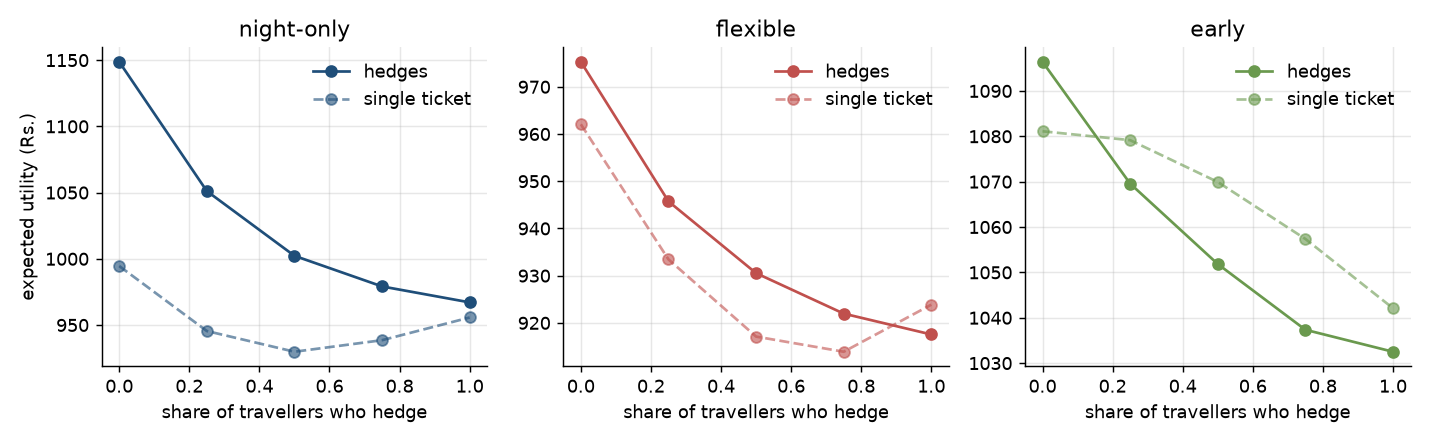
\includegraphics[width=\textwidth]{q1_dilemma.png}
\caption{What a hedge and a single ticket are worth to each type, as more travellers hedge.}
\label{fig:q1}
\end{figure}

For the night-only type, yes. Figure~\ref{fig:q1} shows that the hedge beats a single
ticket whatever the others do, by \rs154 when nobody else hedges and by \rs11 when
everybody does. But the type ends up with \rs967 when everybody hedges against \rs995 when
nobody does. The other two types are not in a dilemma, because for them hedging is not
always the better choice: the flexible type gains about \rs13 until most others hedge and
then loses, and the early type gains only when nobody else hedges. Both are hurt by other
people's hedging, the flexible type falling from \rs962 to \rs918 and the early type from
\rs1,081 to \rs1,033.

In equilibrium every night-only traveller hedges with two tickets, about 40\% of the
flexible type do, and the early type does not. That is 23\% of travellers booking more than one
ticket. Nobody can gain more than a rupee by switching.

\subsection{Hedging or late release?}

\begin{table}[ht]
\caption{The four baselines. Welfare is per season, $\pm450$ to $\pm500$. The travel rate
is among travellers whose plans held.}
\label{tab:q2}
\centering
\begin{tabular}{lcccc}
\toprule
Behaviour & Welfare (\rs) & Travel rate & Empty berths & Turned away \\
\midrule
Nobody hedges & 510,745 & 73.0\% & 1.3\% & 0.0\% \\
All hedge, release on time & 504,380 & 71.8\% & 2.4\% & 14.5\% \\
All hedge, release late & 499,733 & 71.1\% & 3.1\% & 15.5\% \\
Equilibrium & 504,858 & 71.9\% & 2.3\% & 7.8\% \\
Planner who knows all values & 555,615 & & & \\
\bottomrule
\end{tabular}
\end{table}

Going from no hedging to everyone hedging and releasing on time costs \rs6,365 ($\pm221$) a
season. Releasing late costs another \rs4,648 ($\pm199$). So if everyone did both, 58\% of
the loss would be hedging itself and 42\% late release.

Both channels from the introduction show up. Empty berths nearly double with hedging, and
almost all of the increase is travellers who switch to their preferred train after their
backup train has already charted, which is the 6\,pm and 10\,pm example from the introduction.
Hedgers' extra tickets also fill the waitlists, so one traveller in seven gets no ticket at
all. Late release adds berths that go to a redundant ticket at the chart and are then not
used.

The equilibrium row is the surprise. We expected travellers to sit on redundant tickets,
since the clerkage is the same either way. They do not: a redundant ticket that confirms
has to be cancelled at a quarter or half of the fare, and that risk outweighs the hassle.
So in equilibrium the whole loss, \rs5,888 ($\pm211$) or about 1.2\% of welfare, is from
hedging. The planner's much larger gap is a different matter. It comes from berths going
to whoever books first and from the planner knowing whose plans will change.

\subsection{The railway's rules}

For each setting of the rules we recomputed the equilibrium.

\begin{table}[ht]
\caption{Equilibrium under different waitlist caps (Q3).}
\label{tab:q3}
\centering
\begin{tabular}{lcccc}
\toprule
Cap & Hedgers & Tickets per traveller & Turned away & Welfare (\rs) \\
\midrule
10\% & 5.0\% & 0.79 & 25.7\% & 505,944 \\
25\% (June 2025) & 10.5\% & 0.91 & 19.7\% & 505,284 \\
60\% (today) & 23.5\% & 1.16 & 7.8\% & 504,858 \\
none & 35.4\% & 1.35 & 0.0\% & 504,441 \\
\bottomrule
\end{tabular}
\end{table}

\paragraph{Cap (Q3).} A tighter cap cuts hedging a lot (Table~\ref{tab:q3}) but welfare
changes by only \rs1,500 between a 10\% cap and none, because the cap replaces hedging with
refusing people outright. Travellers hold fewer tickets under a tight cap, not more. We
cannot say whether they would book earlier to beat the cap, since arrival times are fixed
in our model, so this answers only half of the ``race for slots'' question.

\begin{figure}[ht]
\centering
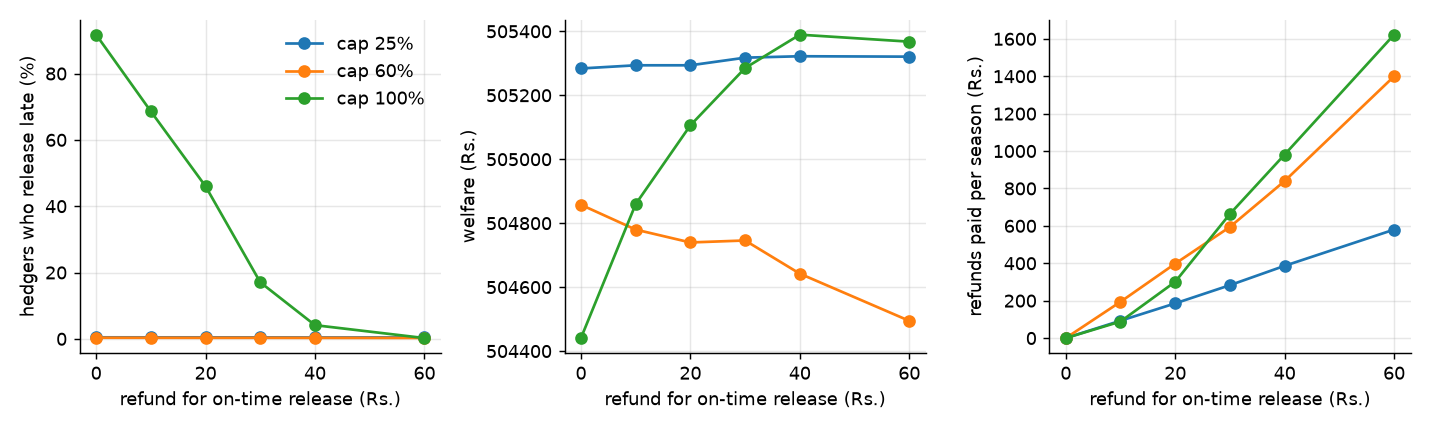
\includegraphics[width=\textwidth]{q4_refund.png}
\caption{A refund for releasing a redundant waitlisted ticket on time, under three caps.}
\label{fig:q4}
\end{figure}

\paragraph{Refund (Q4).} With a 25\% or 60\% cap nobody releases late, so there is nobody for
the refund to persuade (Figure~\ref{fig:q4}). It even does a little harm, because it makes
hedging cheaper: at \rs60 under today's cap, welfare is \rs288 ($\pm90$) lower. Without a cap things are
different. Waitlists get long, a ticket far back is unlikely to confirm, and 92\% of
hedgers release late. A refund of \rs20 brings that down to 46\% and \rs40 to 4\%, for a
welfare gain of about \rs950 a season and about the same amount paid out in refunds. So
under the railway's own objective, which counts refunds as a cost, the \rs40 refund only
breaks even ($-$\rs33), and the best refund is \rs20 ($+$\rs364). The cap and the refund
are substitutes.

\paragraph{Chart time (Q5).} With the chart 4, 8 and 10 hours ahead, 0.8\%, 1.1\% and
1.3\% of berths leave empty when nobody hedges, and 1.8\%, 2.2\% and 2.3\% in equilibrium.
So an earlier chart does leave more berths empty, but through ordinary cancellations that
now fall after the chart. Hedging adds the same 1.1 points every time, because what matters
for switching is the gap between two trains' charts, and that does not change when all
charts move together.

\paragraph{The railway as leader.} Table~\ref{tab:rank} gives the result of the search
over all 36 rule combinations.

\begin{table}[ht]
\caption{Gain over today's rules (60\% cap, no refund, chart 10 h). The best grid point
also has a \rs30 refund, which makes no measurable difference there. Under the railway's
objective the refund rows become $-668$ and $-1{,}682$ and the best row $+3{,}961$; the
others do not change.}
\label{tab:rank}
\centering
\small
\begin{tabular}{lrrrr}
\toprule
Rule & Welfare gain (\rs) & $\pm$ & Railway income (\rs) & Turned away \\
\midrule
Cap 10\% and chart 4 h (best) & $+4{,}088$ & 269 & $-6{,}651$ & 25.9\% \\
Chart 4 h & $+2{,}976$ & 209 & $+1{,}016$ & 8.1\% \\
Cap 10\% & $+1{,}083$ & 201 & $-7{,}301$ & 25.8\% \\
Chart 8 h & $+877$ & 102 & $+307$ & 8.0\% \\
Cap 25\% & $+440$ & 100 & $-4{,}671$ & 19.9\% \\
Refund \rs30 & $-78$ & 46 & $-505$ & 8.5\% \\
Refund \rs60 & $-288$ & 90 & $-1{,}076$ & 9.6\% \\
No cap & $-372$ & 134 & $+3{,}839$ & 0.0\% \\
\bottomrule
\end{tabular}
\end{table}

The chart time is the lever that matters. Moving it from 10 to 4 hours recovers about half
of the loss from hedging and costs the railway nothing. The welfare-best combination adds a
10\% cap, but that turns away a quarter of all travellers and costs the railway income, so
we would not recommend it on these numbers. We should add that our model gives an early
chart no credit for its actual purpose, which is to give waitlisted passengers time to make
other plans.

\subsection{Do Eqs.~(2) and~(3) hold?}
\label{sec:rules}

The review pointed out that Eqs.~(2) and~(3) treat each train's confirmation chance as
fixed and unrelated to the other trains, which is not true in the simulator. We checked
the two assumptions and then the decisions, at five levels of hedging. Counting
confirmations over the whole market would mislead: a ticket its holder cancels early never
shows whether it would have confirmed, and the tickets of travellers who do not hedge sit
deeper in the queue than a hedger's. So we measure the chances on a group of 10\% of
travellers who hedge and are made to hold every ticket until the chart, while everybody
else plays as usual.

\begin{figure}[ht]
\centering
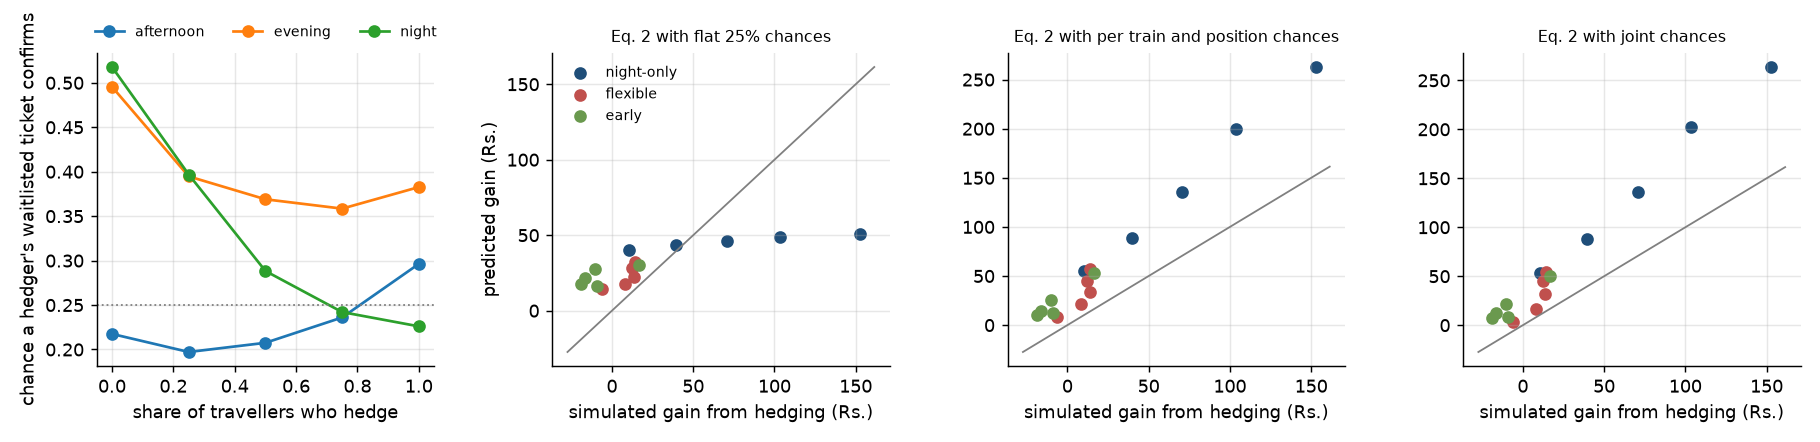
\includegraphics[width=\textwidth]{rule_check.png}
\caption{Left: chance that a hedger's waitlisted ticket confirms, as more travellers hedge.
Right: the gain from a second ticket predicted by Eq.~(2) against the simulated gain, when
the rule is given the flat 25\%, the measured rate per train and queue position, and the
same with the independence assumption replaced by measured joint chances. A perfect
prediction lies on the line.}
\label{fig:rules}
\end{figure}

The chances are not fixed. A hedger's waitlisted ticket on the night train confirms 52\% of
the time when nobody else hedges and 23\% when everybody does (Figure~\ref{fig:rules},
left), because the others' extra tickets are in the same queue. The rate over all
waitlisted tickets in the market moves the other way, from 17\% to 28\%, so even which
chance is meant matters.

They are not independent either (Table~\ref{tab:joint}). Among travellers waitlisted on two
trains, both tickets confirm more often than the product of the two rates at every level
of hedging, and about two and a half times as often when everybody hedges. Someone who
books early is near the front of both queues. The effect is strongest for the early type
(27 to 30\% against 11 to 15\%) and nearly absent for the other two types when
25\% or 50\% of travellers hedge.

\begin{table}[ht]
\caption{Travellers waitlisted on two trains who hold both tickets to the chart.}
\label{tab:joint}
\centering
\small
\begin{tabular}{lccccc}
\toprule
Share of travellers who hedge & 0\% & 25\% & 50\% & 75\% & 100\% \\
\midrule
Better ticket confirms & 20.4\% & 15.1\% & 15.5\% & 20.3\% & 29.3\% \\
Backup ticket confirms & 42.4\% & 34.9\% & 33.8\% & 32.7\% & 33.5\% \\
Both confirm & 14.0\% & 9.2\% & 9.7\% & 14.7\% & 24.8\% \\
Both confirm, if independent & 8.6\% & 5.3\% & 5.2\% & 6.6\% & 9.8\% \\
\bottomrule
\end{tabular}
\end{table}

For the decisions, we compared the gain each rule predicts with the gain in the simulation,
for three types at five levels of hedging. Eq.~(3) does well: it recommends the right
release decision in 14 of 15 cases, and in the one miss the simulated gain is close to
zero. Eq.~(2) is right in only 10 of 15. It always predicts that a second ticket pays, and
for the early type it usually does not. Better chances do not help. The average error is
\rs29 with the flat 25\%, \rs32 with the measured rate per train and \rs43 with the rate
per train and queue position. Replacing the product in Eq.~(2) by the measured joint
chances brings that to \rs41. It lowers the predicted gain for the early type at every level of
hedging and for the flexible type at four of the five, which is the right direction, but
by too little to change any of the 15 decisions.
So neither the fixed chances nor independence is what is wrong with Eq.~(2). What it misses is timing. It values every confirmation at the
full step up to the better train, but some upgrades confirm only after the backup train
has charted, when at least half of the backup's fare is gone, and others are given up
before they confirm. A better rule would split the confirmation chance by when the
confirmation arrives. We did not build one.

\subsection{Travellers who learn}

In the equilibrium analysis travellers know what each strategy is worth. Here they start
knowing nothing and learn it over 8,000 seasons.

\begin{table}[ht]
\caption{Three kinds of traveller and the fixed baselines in the same market, on seasons
not used for training. The rule-followers are given the true confirmation chances. Welfare
is $\pm470$ to $\pm500$.}
\label{tab:learn}
\centering
\small
\begin{tabular}{lcccc}
\toprule
Population & Hedgers & Turned away & Utility (\rs) & Welfare (\rs) \\
\midrule
Equilibrium & 23.3\% & 8.0\% & 970 & 505,345 \\
Follow Eqs.~(2) and (3) & 17.8\% & 3.4\% & 969 & 505,829 \\
Learners (three runs) & 14 to 15\% & 1.5 to 2.1\% & 972 to 974 & 505,778 to 506,214 \\
\midrule
All hedge, release on time & 31.3\% & 14.7\% & 961 & 504,937 \\
All hedge, release late & 29.9\% & 15.7\% & 954 & 500,484 \\
Nobody hedges & 0\% & 0.0\% & 1,000 & 511,184 \\
\bottomrule
\end{tabular}
\end{table}

The learners end up close to the equilibrium in welfare and utility, a little above it
(Table~\ref{tab:learn}), and three independent training runs agree with each other.
Travellers who follow Eqs.~(2) and~(3) land in the same range. In welfare all of them are
only a little better than everybody hedging and releasing on time, and far below nobody
hedging. Where they differ is in how many travellers hedge and how many are turned away,
and the learners get there with the least hedging.
A learner can make her choice depend on the queue she
sees, which none of our five fixed strategies can, and she uses that. She releases a
redundant ticket when it is in the first six places of the queue, where it is likely to
confirm, and mostly holds it when it is further back with the chart less than a day away.
That is the logic of Eq.~(3), found without being told the confirmation chances.

\subsection{How far to trust this}
\label{sec:trust}

\begin{figure}[ht]
\centering
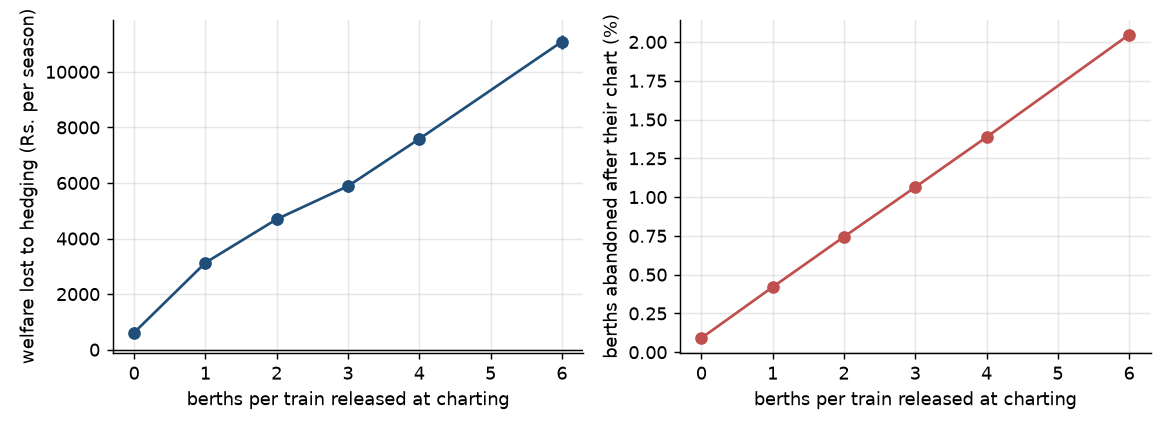
\includegraphics[width=0.8\textwidth]{chart_release.png}
\caption{Welfare lost to hedging in equilibrium, and berths abandoned after their chart,
against the number of berths per train that reach the waitlist only at charting.}
\label{fig:quota}
\end{figure}

The size of the harm depends heavily on the berths released at charting
(Figure~\ref{fig:quota}). With none, hedging costs \rs613 a season. With our default of
three it costs \rs5,888, and with six \rs11,086, while the number of hedgers hardly
changes. So the mechanism is solid but the magnitude is not. Hedging does harm when a
confirmation arrives after the hedger's backup train has charted, and how often that
happens depends on how many berths the railway releases late. Emergency quota is reported
to be about 18 berths per train in AC 3-tier~\cite{eq}, a few percent of capacity, but we
could not find how much of it goes unused. The 1.2\% figure should be read with that in
mind.

The other assumptions matter less. Moving demand, the plan-change rate, the resale chance,
the hassle cost, the outside option, the spread of values and the cost of an empty berth
each down and up keeps the share of hedgers between 17\% and 26\% and the equilibrium loss
between \rs4,750 and \rs7,900.

On the equilibrium itself we ran two checks. Starting best-response iteration from an even
mix, from nobody hedging and from everyone hedging late gives the same profile each time.
And since our deviating group is 10\% of travellers, not the single traveller of the Nash
definition, we repeated the search with a 3\% group and with one traveller. The result is
the same: the night-only type hedges, 41 to 47\% of the flexible type hedge, and no type
can gain more than \rs3 by switching. The largest regret in every run is the flexible
type's (\rs0.8 to \rs2.8); the other two types are below \rs0.4. This is why we call the
result an approximate equilibrium between types and not an exact Nash equilibrium.

Some things the model cannot say. Travellers' values are invented, since there is no public
booking data. Arrival times are fixed, so we cannot see travellers booking earlier.
Everyone has the same outside option. And the clerkage and the quota size come from press
reports, not official documents.

\section{Conclusion}

Hedging is rational for travellers who care a lot about one train, and it leaves them and
everyone else worse off. The damage is not so much that hedgers hold extra tickets, and
with today's charges it is not that they release them late. It is that some confirmations
come after the hedger's backup train has charted, when the backup berth can no longer be
passed on. That is why the chart time and the berths released at charting matter more in
our results than the cap or a refund.

\section{Contribution}

\begin{center}
\small
\begin{tabular}{lp{0.6\textwidth}l}
\toprule
Member & Assigned task & Status \\
\midrule
Akshit Chhabra & Model design, booking simulator, welfare accounting, policy experiments
(Q1 to Q5), putting the pieces together & Completed \\
Kunal Chandola & Equilibrium solver and its robustness checks, search over the railway's
rules & Completed \\
Miloni Thakkar & Check of Eqs.~2 and~3, verifying policy facts against current sources,
report & Completed \\
Devarshi Savalgi & Learning travellers (Monte Carlo control), their comparison with the
equilibrium and the rule-followers, tests & Completed \\
\bottomrule
\end{tabular}
\end{center}

\begin{thebibliography}{99}\small

\bibitem{rs} Devdiscourse (PTI). ``Railways' strategy to tackle waitlisted passengers.''
December 2024. \url{https://www.devdiscourse.com/article/business/3178763-railways-strategy-to-tackle-waitlisted-passengers}

\bibitem{quarter} Udaipur Times. ``Railway limits waiting list tickets.'' 21 June 2025.
\url{https://udaipurtimes.com/travel-and-tourism/railway-limits-waiting-list-tickets/cid16938911.htm}

\bibitem{cap} Free Press Journal. ``Railway Board revises 25\% cap on waiting list tickets
following public outcry.'' 30 June 2025.
\url{https://www.freepressjournal.in/india/railway-board-revises-25-cap-on-waiting-list-tickets-following-public-outcry}

\bibitem{chart10} DT Next. ``First reservation chart to be released 10 hours in advance.''
19 December 2025.
\url{https://www.dtnext.in/amp/story/news/national/first-reservation-chart-to-be-released-10-hours-in-advance-aadhar-authenticated-booking-time-extended-railway-board}

\bibitem{slabs} All India Radio News. ``Railways Minister Ashwini Vaishnaw launches five
reforms in Railways.'' 24 March 2026.
\url{https://www.newsonair.gov.in/railways-minister-ashwini-vaishnaw-launches-five-reforms-in-railways-52-reforms-in-52-weeks-drive}

\bibitem{irctc} IRCTC. ``Procedure for cancellation of e-tickets.''
\url{https://contents.irctc.co.in/en/eticketCancel.html}

\bibitem{clerkage} Business Today. ``Before you cancel your train ticket, check these new
refund rules by Indian Railways.'' 28 March 2026.
\url{https://www.businesstoday.in/india/story/before-you-cancel-your-train-ticket-check-these-new-refund-rules-by-indian-railways-522453-2026-03-28}

\bibitem{fare} ConfirmTkt. Seat availability and fares, 12230 Lucknow Mail.
\url{https://www.confirmtkt.com/train-seat-availability/12230-lucknow-mail}

\bibitem{eq} OneIndia. ``Emergency quota in train: FAQs.''
\url{https://www.oneindia.com/india/emergency-quota-in-train-faqs-how-many-seats-are-reserved-who-can-apply-and-what-indian-railways-7990949.html}

\bibitem{talluri} K. T. Talluri and G. J. van Ryzin. \emph{The Theory and Practice of
Revenue Management}. Springer, 2004.

\end{thebibliography}

\end{document}
